\chapter{Funciones}\label{funciones}

La función es, tal vez, uno de los conceptos más importantes en matemáticas, pues gran parte de los demás conceptos matemáticos se basan en el conocimiento de las funciones y sus propiedades. Aunque existen muchos tipos de funciones —por ejemplo, el área de un círculo que depende de su radio, el costo de un envío que depende de su peso, o la velocidad que depende del tiempo \(t\) transcurrido—, las funciones no siempre dependen de una sola variable. Por ejemplo, el volumen de un cilindro depende tanto de su altura como de su radio. 

En esta sección nos enfocaremos inicialmente en las funciones de una variable real y desarrollaremos con detalle este concepto fundamental.


\section{Propiedades básicas}

\begin{definition}[Función]
Una función \( f \) es una regla de correspondencia que asigna a cada elemento \( x \) de un conjunto denominado \textbf{dominio}, un único valor \( f(x) \) en otro conjunto, llamado \textbf{codominio}. 

El conjunto de todos los valores \( f(x) \) obtenidos se denomina \textbf{rango} o \textbf{imagen} de \( f \). Es común decir que $x$ es la variable independiente y $f(x)$ es la variable dependiente además de usar la notación $y=f(x)$ de manera indistinta.
\end{definition}
\begin{prob} 
Calcule el dominio de las siguientes funciones
\begin{enumerate}
\item $f(x)=x^2-8x+5.$
\item $f(x)=\sqrt{1-x^2}.$
\item $f(x)=\sqrt{3+x}+\sqrt[4]{7-x}.$
\item $f(x)=\dfrac{x+5}{x-3}$
\end{enumerate}
\begin{myproof}
\begin{enumerate}
\item La función es un polinomio de grado $2$. Los polinomios están definidos para todo $x \in \mathbb{R}$, sin restricciones. Por tanto, \(
\operatorname{Dom}(f) = \mathbb{R}.
\)
\item La raíz cuadrada requiere que su argumento sea no negativo, es decir
\[
1 - x^2 \geq 0 \iff x^2 \leq 1 \iff -1 \leq x \leq 1.
\]
No hay otras restricciones. Por tanto, \(
\operatorname{Dom}(f) = [-1, 1].
\)
\item Analizamos cada radical por separado. Para $\sqrt{3+x}$ se cumple que $3 + x \geq 0 \iff x \geq -3$ y para $\sqrt[4]{7-x}$ se tiene que las raíces de índice par requieren radicando $\geq 0$. Así, $7 - x \geq 0 \iff x \leq 7$. Finalmente la suma está definida cuando ambas lo están, por tanto 
\(\operatorname{Dom}(f) = [-3, 7].\)
\item La función está definida para todo número real excepto donde el denominador sea 0. De esta manera, \(\operatorname{Dom}(f) = \mathbb{R}-\lbrace 3 \rbrace.\)
\end{enumerate}
\end{myproof}
\end{prob}


\begin{rem}[Formas de representar una función]
Existen básicamente cuatro formas de representar una función: verbalmente, describiendo en palabras la relación entre variables; numéricamente, mediante una tabla de valores; visualmente, a través de una gráfica; y algebraicamente, por medio de una fórmula explícita. Aclararemos estas formas en el siguiente ejemplo.
\end{rem}

\begin{example}\label{funcioncosto}
Un contenedor rectangular sin tapa tiene un volumen de \(10\,\text{m}^3\). La longitud de su base es dos veces su ancho. El material para la base cuesta \$10 por metro cuadrado y el material para los lados cuesta \$6 por metro cuadrado. Exprese el costo de los materiales como una función del ancho de la base. Dé una representación verbal, numérica, visual y algebraica.

\begin{myproof}
Primero introducimos las variables geométricas del problema. Sea \(x\) el ancho de la base (en metros), \(2x\) la longitud de la base (en metros) y \(h\) la altura del contenedor (en metros). Como el contenedor no tiene tapa, solo hay base y cuatro lados.

La condición de volumen se escribe como
\[
V = (\text{ancho})\cdot(\text{longitud})\cdot(\text{altura}) = x \cdot 2x \cdot h = 2x^{2}h = 10.
\]
Despejamos la altura en función del ancho:
\[
h = \frac{10}{2x^{2}} = \frac{5}{x^{2}}.
\]

Ahora calculamos el área de cada parte para expresar el costo total. 
El área de la base es
\[
A_{\text{base}} = x \cdot 2x = 2x^{2},
\]
y su costo es
\[
C_{\text{base}} = 10 \cdot A_{\text{base}} = 10 \cdot 2x^{2} = 20x^{2}.
\]

El contenedor tiene cuatro lados rectangulares: dos lados de dimensiones \(x \times h\) y dos de dimensiones \(2x \times h\). El área total de los lados es
\[
A_{\text{lados}} = 2(xh) + 2(2xh) = 2xh + 4xh = 6xh.
\]
Sustituimos \(h = \dfrac{5}{x^{2}}\):
\[
A_{\text{lados}} = 6x \cdot \frac{5}{x^{2}} = \frac{30}{x}.
\]
El costo de los lados es entonces
\[
C_{\text{lados}} = 6 \cdot A_{\text{lados}} = 6 \cdot \frac{30}{x} = \frac{180}{x}.
\]

Sumando ambos aportes obtenemos el costo total como función del ancho \(x\):
\[
C(x) = C_{\text{base}} + C_{\text{lados}} = 20x^{2} + \frac{180}{x}.
\]

Podemos ahora presentar las cuatro representaciones de la función costo:

\textbf{Representación verbal:} A cada valor positivo del ancho \(x\) se le asigna el costo total de construir el contenedor, sumando el costo de la base y el de los cuatro lados, donde la longitud es \(2x\) y la altura se ajusta para que el volumen sea \(10\,\text{m}^3\).

\textbf{Representación algebraica:} La función costo en términos del ancho \(x\) está dada por
\[
C(x) = 20x^{2} + \frac{180}{x}, \quad x > 0.
\]

\textbf{Representación numérica:} Podemos elaborar una tabla de valores, eligiendo algunos anchos \(x\) (en metros) y calculando el costo \(C(x)\) (en dólares). Por ejemplo:
\[
\begin{array}{c|c}
x & C(x) \\
\hline
1   & 20(1)^{2} + \dfrac{180}{1}   = 200 \\
1.5 & 20(1.5)^{2} + \dfrac{180}{1.5} = 20\cdot 2.25 + 120 = 165 \\
2   & 20(2)^{2} + \dfrac{180}{2}   = 80 + 90 = 170 \\
2.5 & 20(2.5)^{2} + \dfrac{180}{2.5} = 20\cdot 6.25 + 72 = 197 \\
\end{array}
\]

\textbf{Representación visual:} La representación gráfica consiste en dibujar la curva de la función
\[
y = C(x) = 20x^{2} + \frac{180}{x}, \quad x > 0,
\]
en el plano \(xy\), donde el eje horizontal representa el ancho \(x\) y el eje vertical representa el costo \(C(x)\). Esta gráfica muestra cómo varía el costo total según el ancho de la base.
\begin{figure}[H]
\centering
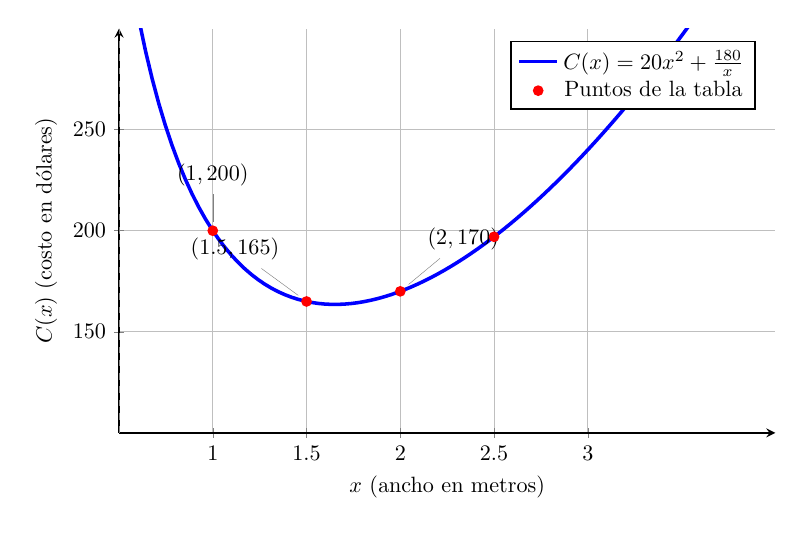
\begin{tikzpicture}[scale=0.8]
% Definir la función
\begin{axis}[
    width=12cm,
    height=8cm,
    xlabel={$x$ (ancho en metros)},
    ylabel={$C(x)$ (costo en dólares)},
    xmin=0.5, xmax=4,
    ymin=100, ymax=300,
    grid=major,
    axis lines=left,
    xtick={1,1.5,2,2.5,3},
    ytick={150,200,250},
    legend pos=north east,
    domain=0.5:4,
    samples=100,
    thick
]

% Graficar la función C(x)
\addplot[blue, ultra thick] {20*x^2 + 180/x};
\addlegendentry{$C(x)=20x^2+\frac{180}{x}$}

% Marcar los puntos de la tabla numérica
\addplot[red, mark=*, only marks] coordinates {
    (1,200)
    (1.5,165)
    (2,170)
    (2.5,197)
};
\addlegendentry{Puntos de la tabla}

% Etiquetas de los puntos clave
\node[pin=90:{$(1,200)$}] at (axis cs:1,200) {};
\node[pin=120:{$(1.5,165)$}] at (axis cs:1.5,165) {};
\node[pin=60:{$(2,170)$}] at (axis cs:2,170) {};

% Línea vertical en x=0 (asíntota)
\draw[dashed, gray] (axis cs:0.5,100) -- (axis cs:0.5,300) node[above right] {asíntota};

\end{axis}
\end{tikzpicture}
\caption{Figura del ejemplo \ref{funcioncosto}}

\end{figure}
Con esto hemos descrito el costo como función del ancho en sus cuatro formas: verbal, numérica, visual y algebraica.
\end{myproof}
\end{example}
Aunque conocer las cuatro representaciones de una función (verbal, numérica, algebraica y gráfica) es fundamental, en ocasiones una resulta más conveniente que las demás según el contexto. Por ello, es esencial seleccionar la representación más adecuada para cada situación particular. La siguiente es una propiedad clave para identificar gráficas de funciones:

\begin{rem}[Prueba de la recta vertical]

\begin{multicols}{2}
Una curva en el plano $XY$ es la gráfica de una función $y=f(x)$ si y solo si ninguna recta vertical se interseca con la curva en más de un punto. 

Por ejemplo, la circunferencia de radio $1$ centrada en el origen, dada por $x^2 + y^2 = 1$, no representa una función de $x$, ya que una recta vertical como $x=0.5$ la interseca dos veces.

\begin{figure}[H]
\centering
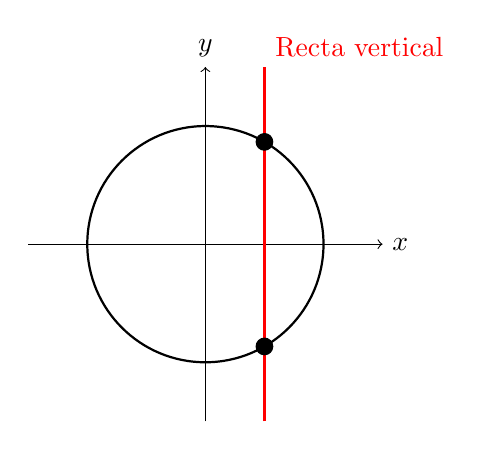
\begin{tikzpicture}[scale=1.5]
\draw[->] (-1.5,0) -- (1.5,0) node[right] {$x$};
\draw[->] (0,-1.5) -- (0,1.5) node[above] {$y$};
\draw[thick] (0,0) circle (1cm);
\draw[red, very thick] (0.5, -1.5) -- (0.5,1.5) node[above right] {Recta vertical};
\filldraw (0.5, 0.866) circle (2pt) node[above right] {};
\filldraw (0.5, -0.866) circle (2pt) node[below right] {};
\end{tikzpicture}
\caption{Circunferencia unitaria fallando la prueba de la recta vertical.}
\label{fig:circulo-vertical}
\end{figure}
\end{multicols}
\end{rem}

\begin{definition}[Funciones crecientes y decrecientes] Una función $f$ se denomina \textbf{creciente} sobre un intervalo $I$ si $f(x_1)<f(x_2)$ siempre que $x_1<x_2$ para todo $x\in I.$ De manera análoga $f$ se denomina \textbf{decreciente} sobre un intervalo $I$ si $f(x_1)>f(x_2)$ siempre que $x_1<x_2\in I.$
\end{definition}

\begin{example} 
Determine los intervalos donde la función $f(x)=x^2$ es creciente o decreciente.
\begin{myproof} Hagamos inicialmente un bosquejo de la función

\begin{figure}[H]
\centering
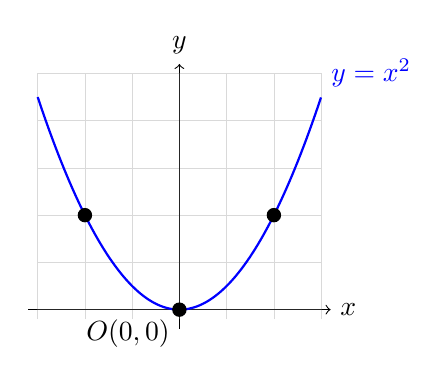
\begin{tikzpicture}[scale=1.2]
% Ejes
\draw[->] (-1.6,0) -- (1.6,0) node[right] {$x$};
\draw[->] (0,-0.2) -- (0,2.6) node[above] {$y$};

% Malla ligera cerca de cero
\draw[help lines, step=0.5cm, opacity=0.3] (-1.5,-0.1) grid (1.5,2.5);

% Bosquejo de y = x^2 cerca de cero
\draw[thick, blue, domain=-1.5:1.5, samples=100] plot (\x, {\x*\x}) 
    node[above right] {$y = x^2$};

% Puntos clave cerca de cero
\filldraw (0,0) circle (2pt) node[below left] {$O(0,0)$};
\filldraw (1,1) circle (2pt) node[above right] {};
\filldraw (-1,1) circle (2pt) node[above left] {};

\end{tikzpicture}
\caption{Bosquejo de $y=x^2.$}
\label{fig:parabola-cero}
\end{figure}


Visualmente se observa que la función tiene forma de parábola y vértice en $x=0$, sugiriendo comportamiento diferente a cada lado. Analizamos por casos.

\textbf{Caso 1: $x \geq 0$ (intervalo $[0, +\infty)$).} Sean $x_1, x_2 \geq 0$ con $x_1 < x_2$. Entonces $x_2 - x_1 > 0$.

Calculamos:
\begin{align*}
f(x_2) - f(x_1) &= x_2^2 - x_1^2 = (x_2 - x_1)(x_2 + x_1).
\end{align*}
Como $x_2 - x_1 > 0$ y $x_2 + x_1 \geq x_1 + x_1 = 2x_1 \geq 0$, se tiene $f(x_2) - f(x_1) > 0 \iff f(x_2) > f(x_1)$.

Por tanto, $f$ es estrictamente creciente en $[0, +\infty)$.


\textbf{Caso 2: $x \leq 0$ (intervalo $(-\infty, 0]$).} Sean $x_1, x_2 \leq 0$ con $x_1 < x_2 \leq 0$. Entonces $x_2 - x_1 > 0$.

Ahora:
\begin{align*}
f(x_2) - f(x_1) &= x_2^2 - x_1^2 = (x_2 - x_1)(x_2 + x_1).
\end{align*}
Como $x_2 - x_1 > 0$ pero $x_2 + x_1 \leq x_2 + x_2 = 2x_2 \leq 0$, se tiene $f(x_2) - f(x_1) < 0 \iff f(x_2) < f(x_1)$.

Por tanto, $f$ es estrictamente decreciente en $(-\infty, 0]$.

\end{myproof}
\end{example}

El ejemplo anterior se resolverá con mayor facilidad más adelante, luego de estudiar la derivada. Mientras tanto, observe que hay algunas formas adicionales de representar funciones:

\begin{example}[Función definida por partes] 
A veces las funciones se describen mediante diferentes fórmulas o expresiones en distintas partes de sus dominios. Trace la gráfica de la siguiente función definida por partes: 
\[
f(x) = 
\begin{cases}
3-\dfrac{1}{2}x & \text{si } x < 2 \\
2x-5 & \text{si } x \geq 2 \\
\end{cases}
\]
\begin{myproof}
El dominio de la función es $\mathbb{R}$. Graficamos cada pieza por separado: Para $x<2$: $y=3 - \frac{1}{2}x$ es recta decreciente con pendiente $-\frac{1}{2}$, círculo \textbf{abierto} en $x=2$ ($y=2$) y para $x \geq 2$: $y=2x-5$ es recta creciente con pendiente $2$, círculo \textbf{lleno} en $x=2$ ($y=-1$).

\begin{figure}[H]
\centering
\begin{tikzpicture}[scale=1.2]
\draw[->] (0, -2) -- (0, 4) node[right] {$y$};
\draw[->] (-0.5, 0) -- (4.5, 0) node[right] {$x$};
\node at (2, -0.3) {$2$};

% Rama 1: x < 2, 3 - 0.5x (círculo abierto en x=2)
\draw[thick, blue, domain=-0.5:1.99, samples=50] plot (\x, {3 - 0.5*\x});
\fill[white, opacity=1] (2,2) circle (3pt); % Círculo abierto
\draw[blue] (2,2) circle (3pt);

% Rama 2: x >= 2, 2x-5 (círculo lleno en x=2)
\draw[thick, red, domain=2:4.5, samples=50] plot (\x, {2*\x - 5});
\filldraw[red] (2,-1) circle (3pt);

\node[blue] at (1,3.2) {$3 - \frac{1}{2}x$ ($x<2$)};
\node[red] at (3.5,2) {$2x-5$ ($x \geq 2$)};
\end{tikzpicture}
\caption{Gráfica de la función $f(x)$ definida por partes.}
\end{figure}
\end{myproof}
\end{example}

\begin{definition}[Funciones pares e impares]
Una función $f: D \to \mathbb{R}$ se denomina \textbf{par} si satisface la condición de simetría respecto al eje $y$:
\[
f(-x) = f(x) \quad \forall x \in D \cap (-D) \neq \emptyset.
\]
Análogamente, se denomina \textbf{impar} si satisface la condición de simetría respecto al origen:
\[
f(-x) = -f(x) \quad \forall x \in D \cap (-D) \neq \emptyset,
\]
donde $D \cap (-D) \neq \emptyset$ garantiza que el dominio sea simétrico respecto al origen o contenga al menos pares simétricos.
\end{definition}

\begin{example}
La función $f(x) = x^2$ es par, ya que:
\[
f(-x) = (-x)^2 = x^2 = f(x) \quad \forall x \in \mathbb{R}.
\]
Asimismo, la función $f(x) = x^3$ es impar, pues:
\[
f(-x) = (-x)^3 = -x^3 = -f(x) \quad \forall x \in \mathbb{R}.
\]
Estas identidades algebraicas verifican las respectivas simetrías geométricas en sus gráficas.
\end{example}

En la sección subsiguiente se presentará un catálogo más completo de funciones elementales, permitiendo explorar sistemáticamente estas propiedades simétricas y otras características relevantes del análisis funcional.



\section{Funciones elementales fundamentales}

Existe un catálogo básico de funciones elementales fundamentales ---conocidas también como \emph{modelos matemáticos esenciales}---, que incluye la función potencia, la exponencial, la logarítmica, las trigonométricas y las trigonométricas inversas. Estas constituyen la base para la construcción de modelos matemáticos más complejos, y en este capítulo se analizarán detalladamente sus dominios, rangos y gráficas.


\begin{definition}[Función potencia]
Sea $r \in \mathbb{Q}$ un número racional escrito en su forma reducida $r = \frac{p}{q}$, donde $p \in \mathbb{Z}$ es un entero y $q \in \mathbb{N}^+$ es un entero positivo con $\gcd(p,q)=1$. La función potencia $f(x) = x^r = \sqrt[q]{x^p}$ tiene dominio que depende de la paridad del denominador $q$ y la señal de $r$:

\begin{itemize}
\item Si $q$ es \textbf{impar}, la raíz $q$-ésima está definida para todo $x \in \mathbb{R}$, por lo que $\operatorname{Dom}(f) = \mathbb{R}$.
\item Si $q$ es \textbf{par}, la raíz $q$-ésima de números negativos no está definida en reales, requiriendo $x^p \geq 0$. Para $p$ impar esto equivale a $x \geq 0$, dando $\operatorname{Dom}(f) = [0, +\infty)$.
\item Si $r < 0$, la expresión involucra división por $x^{-r}$, requiriendo excluir $x=0$: $\operatorname{Dom}(f) = \mathbb{R} \setminus \{0\}$ (o $(0,+\infty)$ si $q$ par).
\end{itemize}

Como casos particulares, para enteros positivos $n \in \mathbb{N}$, $f(x) = x^n$ es un polinomio definido en todo $\mathbb{R}$. Para enteros negativos $n < 0$, $f(x) = x^n = \frac{1}{x^{-n}}$ está definida en $\mathbb{R} \setminus \{0\}$.

Estas reglas garantizan que $x^r$ produzca valores reales para todo $x$ en su dominio respectivo.
\end{definition}





\begin{example}[Ejemplos de funciones potencia elementales] Listamos algunos ejemplos representativos
\begin{figure}[h]
\centering
\begin{tikzpicture}[scale=0.8]
\draw[->] (-2,0) -- (2,0) node[right] {$x$};
\draw[->] (0,-1.5) -- (0,2) node[above] {$y$};
\draw[thick, domain=-1.8:1.8, samples=100] plot (\x, {\x});
\node[above right] at (1.5,1.5) {$f(x)=x$};
\end{tikzpicture}
\caption{$f(x)=x$: $\operatorname{Dom} = \mathbb{R}$.}
\end{figure}


\begin{figure}[H]
\centering
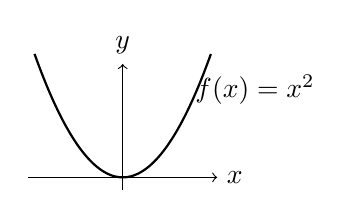
\begin{tikzpicture}[scale=0.8]
\draw[->] (-1.5,0) -- (1.5,0) node[right] {$x$};
\draw[->] (0,-0.2) -- (0,1.8) node[above] {$y$};
\draw[thick, domain=-1.4:1.4, samples=100] plot (\x, {\x*\x});
\node[above right] at (1,1) {$f(x)=x^2$};
\end{tikzpicture}
\caption{Función cuadrática $f(x)=x^2$: $\operatorname{Dom} = \mathbb{R}$.}
\end{figure}

\begin{figure}[H]
\centering
\begin{tikzpicture}[scale=0.8]
\draw[->] (-1.5,0) -- (1.5,0) node[right] {$x$};
\draw[->] (0,-1.2) -- (0,1.8) node[above] {$y$};
\draw[thick, domain=-1.4:1.4, samples=100] plot (\x, {\x*\x*\x});
\node[above right] at (1,1) {$f(x)=x^3$};
\end{tikzpicture}
\caption{Función cúbica $f(x)=x^3$: $\operatorname{Dom} = \mathbb{R}$.}
\end{figure}

\begin{figure}[H]
\centering
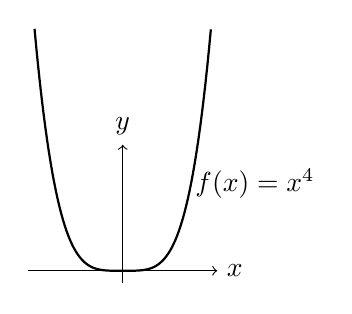
\begin{tikzpicture}[scale=0.8]
\draw[->] (-1.5,0) -- (1.5,0) node[right] {$x$};
\draw[->] (0,-0.2) -- (0,2) node[above] {$y$};
\draw[thick, domain=-1.4:1.4, samples=100] plot (\x, {\x*\x*\x*\x});
\node[above right] at (1,1) {$f(x)=x^4$};
\end{tikzpicture}
\caption{Función $f(x)=x^4$: $\operatorname{Dom} = \mathbb{R}$, par.}
\end{figure}

\begin{figure}[H]
\centering
\begin{tikzpicture}[scale=0.8]
\draw[->] (-2,-2) -- (2,-2) node[right] {$x$};
\draw[->] (0,-2) -- (0,3) node[above] {$y$};
\draw[thick, blue, domain=-1.8:-0.1, samples=100] plot (\x, {1/\x});
\draw[thick, blue, domain=0.1:1.8, samples=100] plot (\x, {1/\x});
\node[blue, above right] at (1.2,1) {$f(x)=1/x$};
\end{tikzpicture}
\caption{Función recíproca $f(x)=1/x$: $\operatorname{Dom} = \mathbb{R} \setminus \{0\}$}
\end{figure}



\begin{figure}[H]
\centering
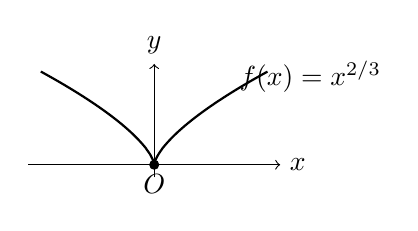
\begin{tikzpicture}[scale=0.8]
\draw[->] (-2,0) -- (2,0) node[right] {$x$};
\draw[->] (0,-0.2) -- (0,1.6) node[above] {$y$};
\draw[thick, domain=-1.8:1.8, samples=200] plot (\x, {abs(\x)^(2/3)});
\filldraw (0,0) circle (2pt) node[below] {$O$};
\node[above right] at (1.2,1) {$f(x)=x^{2/3}$};
\end{tikzpicture}
\caption{Función $x^{2/3}$: $\operatorname{Dom} = \mathbb{R}$.}
\end{figure}

\end{example}











